\documentclass[conference]{IEEEtran}
% \IEEEoverridecommandlockouts
% The preceding line is only needed to identify funding in the first footnote. If that is unneeded, please comment it out.
\usepackage{cite}
\usepackage{amsmath,amssymb,amsfonts}
\usepackage{algorithmic}
\usepackage{graphicx}
\graphicspath{{./images/}}
\usepackage{textcomp}
\usepackage{subfig}
\usepackage{xcolor}
\def\BibTeX{{\rm B\kern-.05em{\sc i\kern-.025em b}\kern-.08em
    T\kern-.1667em\lower.7ex\hbox{E}\kern-.125emX}}
\begin{document}

\title{Investigating the Effect of Dataset Representivity for Image Colourisation}

\author{\IEEEauthorblockN{Andrew Boyley}
\IEEEauthorblockA{\textit{School of Computer Science} \\
\textit{and Applied Mathematics}\\
\textit{University of the Witwatersrand}\\
Johannesburg, South Africa \\
andrew.boyley@students.wits.ac.za}
\and
\IEEEauthorblockN{William Hill} 
\IEEEauthorblockA{\textit{School of Computer Science} \\
\textit{and Applied Mathematics}\\
\textit{University of the Witwatersrand}\\
Johannesburg, South Africa \\
william.hill1@students.wits.ac.za}
\and
\IEEEauthorblockN{Steven James}
\IEEEauthorblockA{\textit{School of Computer Science} \\
\textit{and Applied Mathematics}\\
\textit{University of the Witwatersrand}\\
Johannesburg, South Africa \\
steven.james@wits.ac.za}
}

\maketitle

\begin{abstract}

\end{abstract}

\begin{IEEEkeywords}
deep learning, bias, dataset imbalance, regression, self-supervised learning
\end{IEEEkeywords}

\section{Introduction}

Machine Learning is a tentative endeavour, whereby subtle changes in the learning environment often lead to profound alterations to both the overall effectiveness of the machine learning model and the accuracy of the desired output. 

Such a phenomenon exists when training a model to recognise and colourise aspects of grayscale images: by employing a training dataset with a bias to a particular locale – like an American or a Eurocentric setting, for instance – any sample taken from outside such an area (with particular focus placed on a South African sample) is misrepresented and yields erroneous results, with the produced colourised image being quintessentially different to the intended image.

The identified cause is the lack of diversity in the training datasets because even though various methods can be implemented in the actual model to mitigate this bias, they cannot account for a wholly prejudiced dataset being used initially, particularly a non-South African dataset being used to train a model to operate on a South African sample. 

Therefore, the aim is to investigate what percentage of the training dataset has to be of local origin compared to the international origin of the remainder of the dataset. However, constructing and testing datasets to determine such a goal is both time consuming and expensive in terms of financial and computational resources required. Hence, the approach of image colourisation has been selected as it allows an uncomplicated procedure of collecting publicly-available images of both International and South African settings, thus providing a simple way to build a diverse dataset which does not need to be labelled or require excessive computational time since the machine learning approach required is one of supervised learning where the expected outcome is derived from the images themselves.

Consequently, the refined aim is to investigate the optimal ratio of non-South African images to South African images in the training dataset is such that bias is minimised and the model performs optimally for both sets of images.

\section{Background}

%Explain notation and setup for regression/classification task in general i.e. objective function

%Describe LAB; classes, etc. 

%Describe eval criteria

%Describe neural network, backprop, Insert image if space
\subsection{Colour space}

To make our lives easier, instead of using the typical RGB color space, we use the CIELAB color space. This makes it convenient when seperating the gray and color channels due to the fact that the 'L' channel in LAB is simply the grayscale image. We can then pass this grayscale input (1 x W x H) through our model and compare the output (2 x W x H) to the original 'AB' channels of the image. These 'AB' channels make up the color and simply show the red-green and blue-yellow shift respectively. HSB would be another option when choosing a suitable colour space. In general, the choice of colour space makes no difference to the resulting image that our network produces.

When reading images from our dataset, we first interpret them in the RBG colour space and then proceed to convert them to LAB using tools such as SciKit Learn or OpenCV, both of which contain colour space conversion libraries. 

\subsection{Regression vs Classification}

When colorizing images using a deep learning approach, it is generally easiest to develop our model as a regression problem. Classification would yield better results which are more life-like and saturated whereas regression would lead to output images appearing dull and bland. This is the result of the multi-modality of pictures. There is no clear color for any one image. This leads our model, using an aggregate loss function, to simply find an average color, resulting in a bland image.

\begin{figure}[h!]
    \centering
    \subfloat[Regression]{{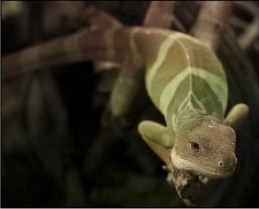
\includegraphics[width=3.5cm]{cham-reg} }}%
    \qquad
    \subfloat[Classification]{{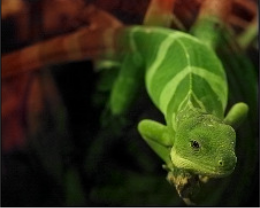
\includegraphics[width=3.5cm]{cham-class} }}%
    \caption{Colour generated using regression vs classification \cite{zhang2016colorful}}%
    \label{fig:reg_vs_class}
\end{figure}

For the sake of simplicity, we continue to use regression as it leads to satisfactory results whilst being simple to understand. We utilize a mean squared error loss which may average color distribution but still produces images with a reasonable amount of color. If we aimed to produce images which were more diverse in colour and saturated, regression would not suffice. Our model should, however, be able to compare output across datasets in order to draw correlation between the accuracy of the ouput and the representivity of local images in the data, which it does.

\subsection{Model topology}

Our choice of model has been based on the simple regression model developed by Luke Melas and loosely based on the network used by Zhang et al. \cite{zhang2016colorful} with the major difference being that their model used in 'Colorful Image Colorization'\cite{zhang2016colorful} approached colorization as a classification problem.

Our network topology consists of the first six layers of a ResNet-18, followed by three layers of deconvolutions. We find that this simple structure works well enough for our purposes and is relatively fast. Our model uses the Adam optimiser alongside PyTorch's autograd which makes backpropogating in our network trivial.

\section{Proposed Method}

%Train colouriser on dataset X. Evaluate accuracy
%
%Explain how our dataset is built precisely: using flickr data, keywords, any preprocessing etc. 
%
%Show some images. 
%
%Maybe even compute mean statistics of dataset X and Y to show that they are in fact different?
%
%Explain method - compute accuracy on X -> X.
%Then check X -> Y
%
%Then check how much of Y must be added to X to improve things?
%
%Would be nice to have multiple datasets, models, but maybe no time :(

\subsection{Brief Outline}

In order to determine the percentage of local data in the training dataset required to mitigate the effect of bias in machine learning models, multiple versions of the dataset are required, with each one consisting of a total of 40000 images and being constructed with a different percentage of South African images from 0\% to 40\% inclusive, increasing in graduations of 10\%. In addition to this training dataset, a validation dataset (of 1000 images in total) is also prepared with the same corresponding percentage inclusion of South African images.

Each version of the dataset will be used to train the model independently of each other for a total of 75 epochs each, with validation being done at the conclusion of each epoch. 

A set collection of South African and International images will be passed through each model respectively, with the subsequent losses being an indication of the bias present in the model due to the predominant locale present in the training images (we take the dataset version with 0\% South African images included as the base case of how the model performs on South African image evaluation when trained exclusively on International images).

\subsection{Building Datasets}

\textbf{Where get european images from?????}

\textbf{and must we show that the datasets are fundamentally different - maybe something that can be said about the source??}

The collection of South African images\footnote{All images are freely available with a Creative Commons Licence or are in the public domain} was downloaded from the image-sharing service, Flickr. Only images which have been tagged with one of the following keywords were selected:

\begin{itemize}
	\item South Africa
	\item Soweto
	\item \textbf{etc. etc.}
\end{itemize}

A Python script was used to assimilate the International and South African images into the required ratios (of 0\% to 40\% South African image inclusion) by selecting the first \emph{n} and \emph{m} images from the image collections, respectively.

\textbf{Include sample images here}

\section{Experiments}

%Explain experiment. Model used. Hyperparameters. Early stopping?? Train/val/test splits.
%
%Show training curves over time for model trained on X. 
%
%Show images from X coloured.
%Show images from Y coloured - qualitative analysis
%
%Start adding data from Y to X. 
%
%Produce THE curve as a function of data ratio
%
%Show images from X coloured.
%Show images from Y coloured - qualitative analysis

\subsection{Training}

For each dataset, we trained our convolutional model from the beginning with the exact same hyperparameters. The following table illustrates the hyperparameters used:


\begin{table}[h]
\centering
\begin{tabular}{|c|c|c|c|}
\hline 
Learning Rate & Epochs & Workers & Batch Size \\ 
\hline 
0.001 & 75 & 4 & 64 \\ 
\hline 
\end{tabular} 
\end{table}

Due to the fact that images collected from Flickr were substantially larger in size than those of the European set, it took longer to train models with a high inclusion rate to the above mentioned epoch. For this reason, we chose to limit our inclusion of South African data to 40\%. Future experiments could show that an inclusion rate higher than 40\% is optimal but for the purpose of this experiment, it will suffice.

For the sake of simplicity, validation and test sets have been merged into one. For each dataset, there are 40000 images in the training set and 1000 in the test/validation split. This makes it an average sized data set which means that inclusions rates on it shoud reflect to others with only minor deviation.

We found that the loss dropped immediately to a reasonable value within the first five epochs but the images produces were not of a high quality. The training process was long and slow with very little change in loss from one epoch to the next but the end results make it worthwhile.

%Insert picures from different epochs

\subsection{Evaluating}

After all models have been trained on their respective datasets, we evaluate them on purely the South African dataset. This gives us a good understanding of how much local data to include into foreign datasets if we want reasonable results. The pure South African dataset contains 35000 images in its training split and 5000 images in the validation/testing split. These were both used to construct the hybrid datasets. Now, we evaluate the model that has been previously trained on the foreign-local hybrid set on a purely South African dataset and measure its performance.

We expect the loss to be much larger when very few South African images have been included into the hybrid set. As we evaluate datasets with a larger inclusion of local data, we expect the models loss to decrease. Using this data, we can estimate the optimal inclusion of local data for satisfactory results when performing machine learning in foreign countries.

After evalutating each model on the same dataset, these are their respective losses,

\begin{table}[h]
\centering
\begin{tabular}{|c|c|c|c|c|}
\hline 
Local inclusion \% & 10\% & 20\% & 30\% & 40\% \\ 
\hline 
Loss & 0.0027 & 0.0027 & 0.0027 & 0.0027 \\ 
\hline 
\end{tabular} 
\end{table}

\section{Related Work}

\begin{itemize}
    \item Find literature on dataset imbalance in general
    \item Find literature on racial bias in general
\end{itemize}

\section{Conclusion}

Important problem

Investigated data representivity

What we found

Extensions to other tasks.

\medskip
 
\bibliographystyle{ieeetr}
\bibliography{bibfile}


% \begin{thebibliography}{00}
% \bibitem{b1} G. Eason, B. Noble, and I. N. Sneddon, ``On certain integrals of Lipschitz-Hankel type involving products of Bessel functions,'' Phil. Trans. Roy. Soc. London, vol. A247, pp. 529--551, April 1955.
% \bibitem{b2} J. Clerk Maxwell, A Treatise on Electricity and Magnetism, 3rd ed., vol. 2. Oxford: Clarendon, 1892, pp.68--73.
% \bibitem{b3} I. S. Jacobs and C. P. Bean, ``Fine particles, thin films and exchange anisotropy,'' in Magnetism, vol. III, G. T. Rado and H. Suhl, Eds. New York: Academic, 1963, pp. 271--350.
% \bibitem{b4} K. Elissa, ``Title of paper if known,'' unpublished.
% \bibitem{b5} R. Nicole, ``Title of paper with only first word capitalized,'' J. Name Stand. Abbrev., in press.
% \bibitem{b6} Y. Yorozu, M. Hirano, K. Oka, and Y. Tagawa, ``Electron spectroscopy studies on magneto-optical media and plastic substrate interface,'' IEEE Transl. J. Magn. Japan, vol. 2, pp. 740--741, August 1987 [Digests 9th Annual Conf. Magnetics Japan, p. 301, 1982].
% \bibitem{b7} M. Young, The Technical Writer's Handbook. Mill Valley, CA: University Science, 1989.
% \end{thebibliography}

\end{document}
